\section{Part I: Data Cleaning and Preprocessing (for dataset A)}
\subsection{Detecting Issues in the dataset}
For this part of the assignment, the dataset had to be analyzed first as part of the preprocessing step to detect issues such as missing values and outliers. There was found to be a 124053 missing values and 14622 outliers in the dataset. Columns and rows that had all NaN values were checked and there was found to be three columns (fea.34, fea.35, fea.36) and 795 rows (samples) that were missing 70\% of the features.
Outliers were found by first finding the standard deviation of each feature and then using each standard deviation to find values in that specific feature that vary by more than 3 standard deviations. 

\subsection{Fixing Issues}
Columns: fea.34, fea.35, fea.36 were dropped from the dataset as they were entirely NaN values. Then the rows (samples) that had all NaN values (795 samples) were dropped from the dataset. After dropping those columns and rows, the number of the missing values reduced from 124,053 to 6048 and the data size reduced to 18205*78 (18205 samples and 78 features). 
After that, the outliers had to be checked and taken care of before replacing the 6048 missing values with the mean as the outliers would effect the mean. There were over 14000 data points (makes ~1 percent of the entire data) that vary from the features mean by over 3 standard deviations. Since the nature of the experiment is not well defined, those outliers are assumed to be noise detected by the motion sensors. After the detection of the outliers, they were replaced with the mean of each feature. Final step was to replace all the missing values denoted by NA with the mean of each feature after the outliers were dealt with. 

\subsection{Normalizing Data}
Figure~\ref{fig:fig1} shows the comparison between histogram plots of feature 9 and 24 before and after normalization. The large spike is a result of multiple data points (outliers and missing values) being set to the mean value as part of the data preprocessing. 
% As it can be seen from the plots below, the only difference between before and after normalization is the scale (range) of the distribution. The distributions curve of both fea.9 and fea.24 did not change before and after applying the normlizations which makes sense as normalization is just a translation or re-scaling the range of the distribution while maintaining the differences in the ranges between the normalized values. In which case this helps us in standardizing the range of the values of different features and comparing them. In this case, looking at the graphs "Before Normalization" in figure 1, it is difficult to compare the two features as the range is not the same.
% Z score normalization: after standardization the data will have zero mean and unit variance
Comparing the two features (9 and 24) from the histogram, we should be able to obtain an idea of the range of the values, mean and standard deviation for each feature. However, looking into the graphs "Before Normalization" in figure 1, we see that it is very difficult to make such a comparison between the features as the range (scale) is different. In this case normalizing the data helps us to better understand the values and make the comparison easier since normalization is just a standardized translation or re-scaling the range of the distribution while maintaining the differences in the ranges between the values. In other words, normalizing data help us to reach a more linear and a robust relationship between the datasets.
\\
To compare the min, max and mid values between fea.9 and fea.24, min-max normalization histogram in figure 1 help us to do so. The min-max normalization range always spans from [0,1] where the minimum value of the feature will be mapped to 0 while maximum value mapped to 1. So the entire range of the values for fea.9 and fea.24 from minimum to maximum are mapped to the range 0 to 1 which makes the comparison easier. We can now comment between the differences between fea.9 and fea.24 where we can notice that fea.9 has more values in the maximum side (higher density) than fea.24 where it looks more like a normal distribution.
\\
The Z-Score normalization is a standardization and re-scaling the range of the data in which the mean is zero and it has a unit variance.
The histogram plot ".. After Z Score Normalization" in figure 1 helps us to compare the spread (standard deviation) of the fea.9 and fea.24. We can see that most values in fea.9 are within a 1 standard deviation. On the other hand, fea.24 has most values spread within 2 standard deviation.
From this analysis, we can concluded that fea.24 looks very similar to a gaussian distribution in terms of the skewness, however, there is a negative kurtosis which deviated from a normal distribution. On the other hand, fea.9 is a multimodal (it has 3 modes) as it can bee seen from the the 3 spikes on the graph. This could imply that there might be different groups or the data could be split into separate groups and could be analyzed further. 

% \begin{itemize}
% \item min/max has range from 0 to 1
% \item z-score is centered around mean = 0 and is ideal for PCA
% \item all histograms have the same shape after cleaning
% \item feat 24 seems to look normally distributed, feat 9 is not
% \end{itemize}


%%%%%%%%%%%%%%%%%%%%%%%%%%%%%%%%%%%%%%%%%%%%%%%%%%%%%%%%%%%%%%%%%%%
%
% Commands to include a figure:
%
%%%%%%%%%%%%%%%%%%%%%%%%%%%%%%%%%%%%%%%%%%%%%%%%%%%%%%%%%%%%%%%%%%%

\begin{figure}[!ht]
 \centering
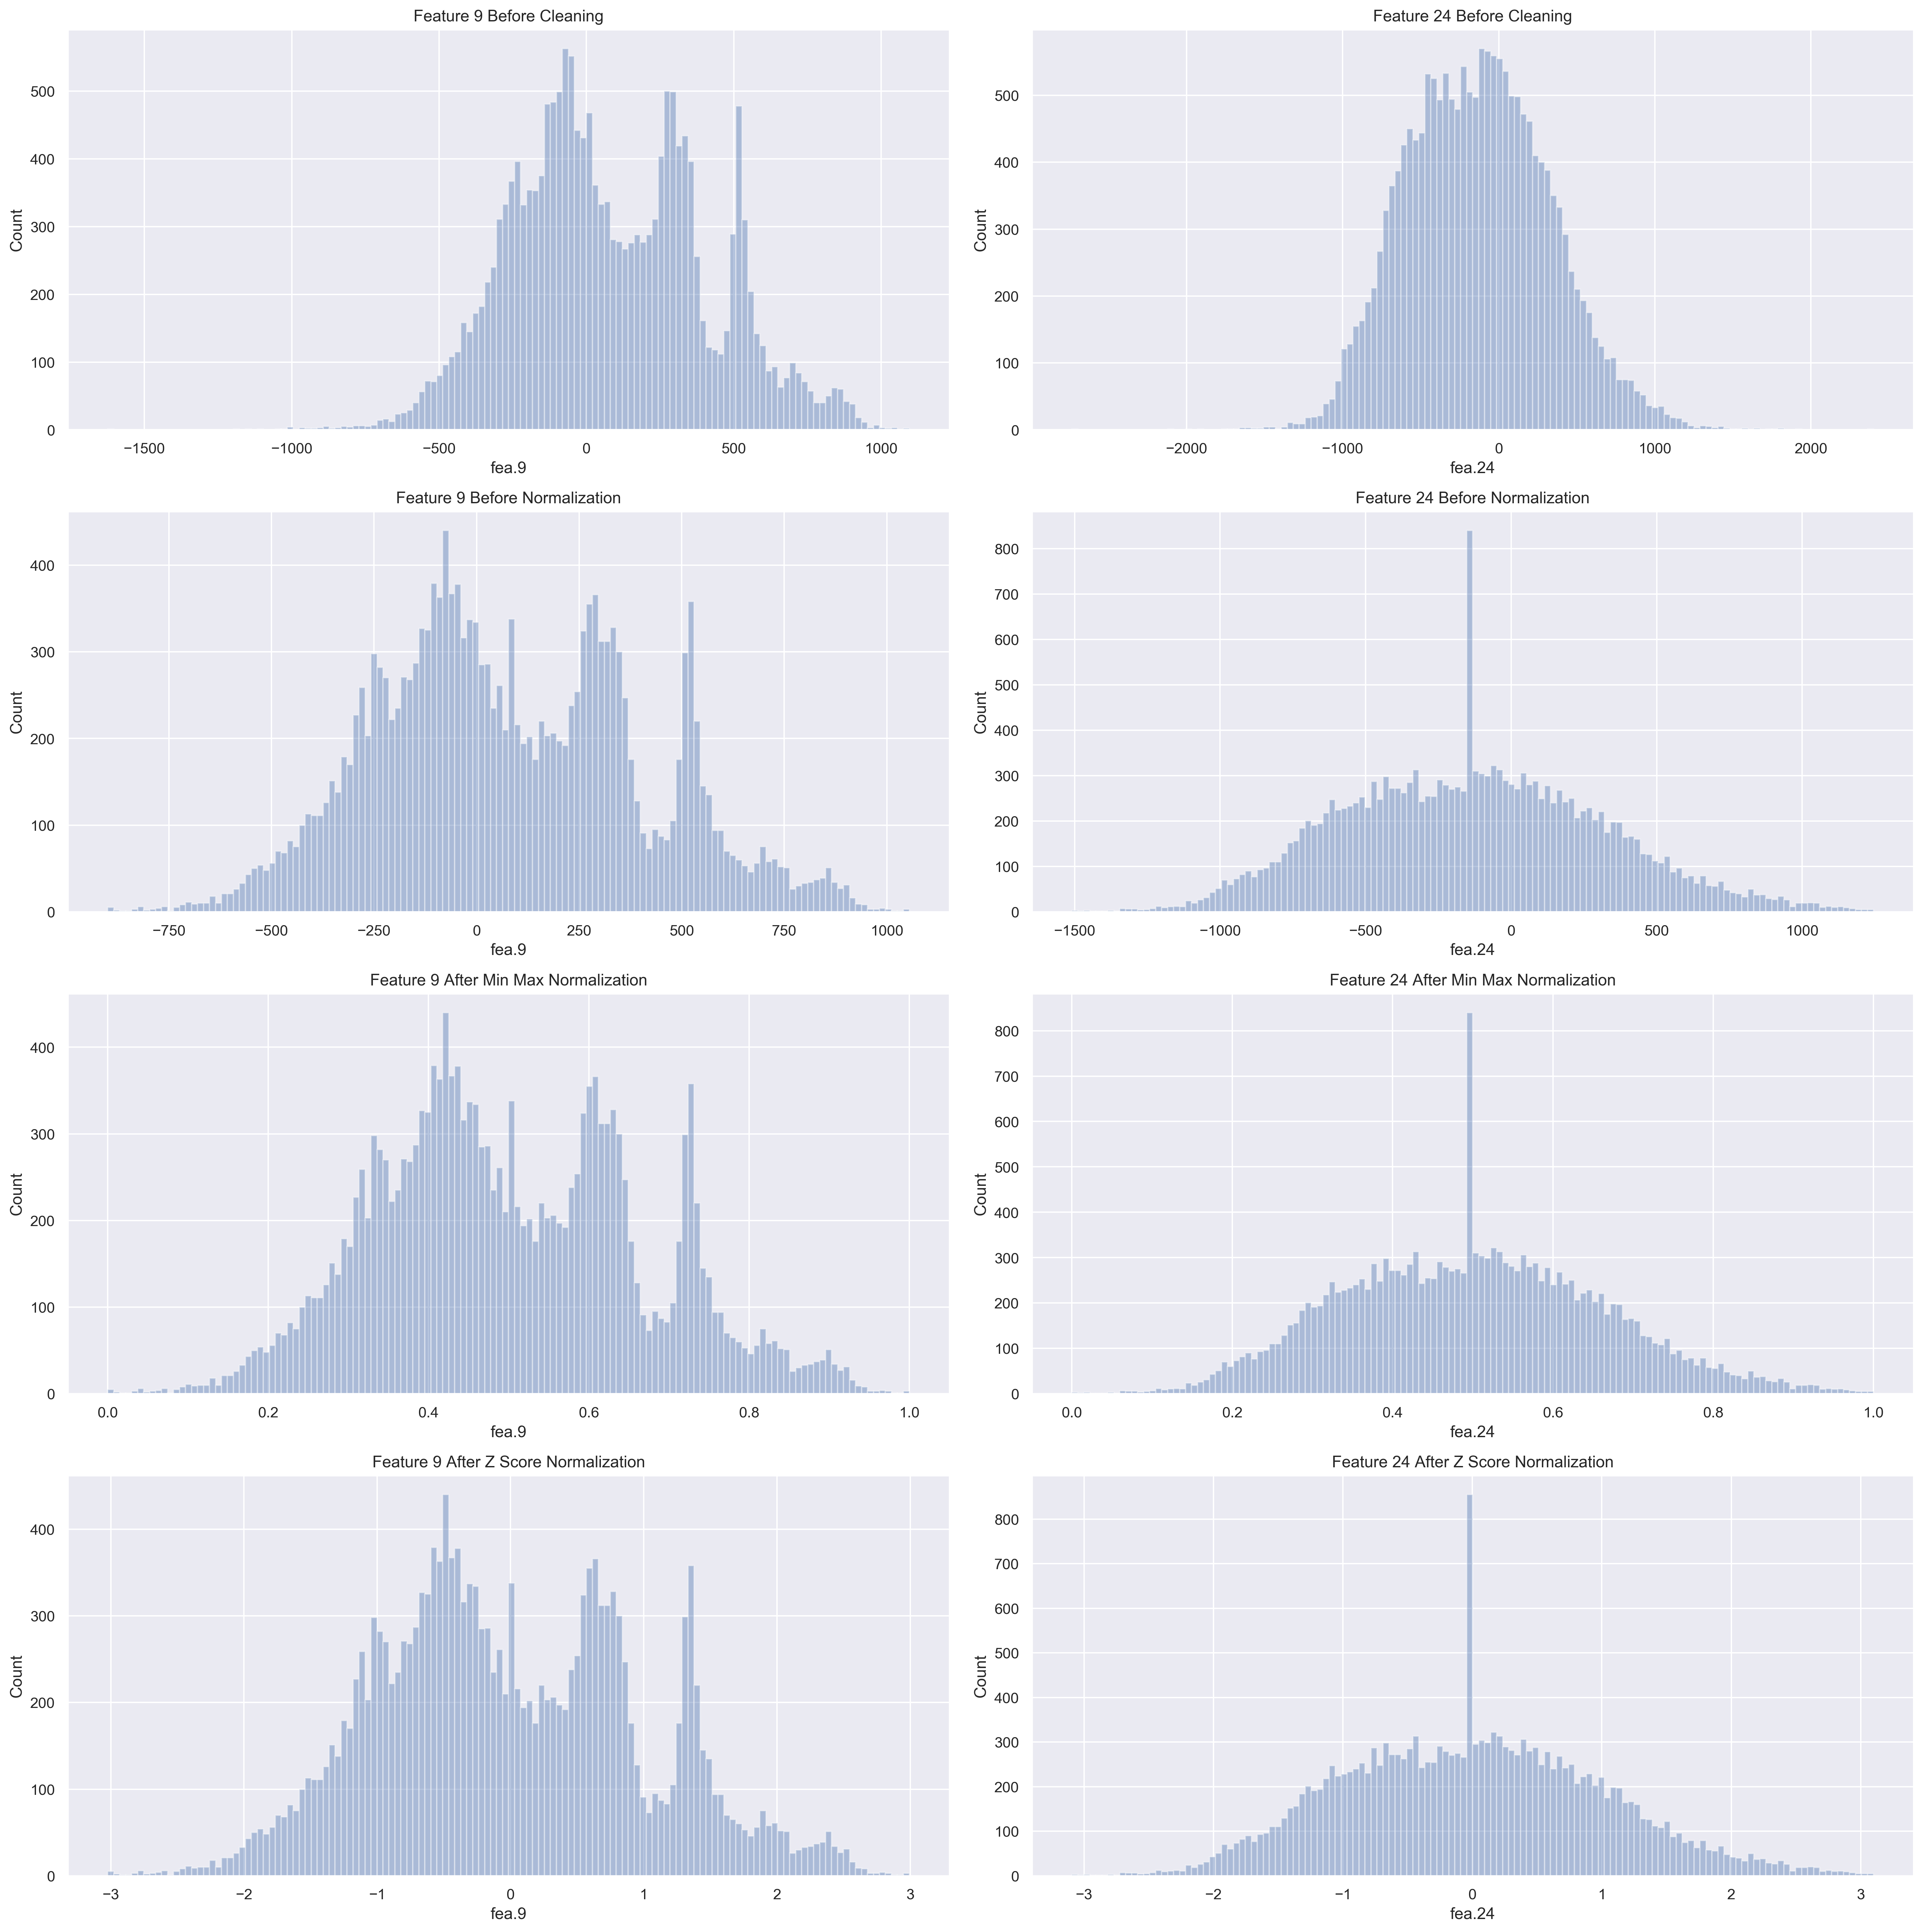
\includegraphics[width=6.1in]{assignment1/1-3-histograms.png}
\caption{\label{fig:fig1}histogram plots of feature 9 and 24 before and after normalization}
\end{figure}
